\chapter{Implementace rozšíření do~webových prohlížečů}\label{chap:extension}

Zatímco podpůrný webový server zajišťuje potřebnou infrastrukturu pro ukládání uživatelských dat, správu uživatelských účtů a rozesílání emailů, klíčovou částí projektu je rozšíření do webových prohlížečů, které zajišťuje integraci přidaných funkcionalit do webového rozhraní školního informačního systému InSIS.

Webové rozšíření jsou softwarové balíčky, které umožňují přidávat nové funkce do webových prohlížečů jako například Google Chrome, Mozilla Firefox nebo Opera. Dále je možné pomocí rozšíření do prohlížečů měnit chování stránek pomocí injekce vlastních skriptů a kaskádových stylů.

Právě prostřednictvím injekce vlastních skriptů a kaskádových stylů jsou implementované funkcionality poskytované rozšířením VŠE+.

\section{Manifest rozšíření}

Základní částí každého rozšíření do webových prohlížečů, bez které nemůže rozšíření vzniknout, je soubor \code{manifest.json}. Jedná se o~konfigurační soubor, který definuje všechny potřebné atributy od názvu rozšíření, popisu, autora až po definice oprávnění a specifikaci přidaných funkcí a skriptů. 

Jednou z~překážek při vývoji rozšíření, která jsou podporována více než jedním webovým prohlížečem je zajištění kompatibility mezi běhovým prostředím a verzí manifestu. Jelikož webový prohlížeč Mozilla Firefox v~době psaní této práce nepodporuje manifest s~verzí 3 a zároveň webové prohlížeče založené na technologii Chrome nepodporuje manifest s~verzí 2, bylo potřeba tyto manifest soubory oddělit do 2 verzí. V~projektu se jedná o~soubory \code{public/manifest-chrome.json} pro webové prohlížeče založené na technologii Chrome a soubor \code{public/manifest-firefox.json} pro webový prohlížeč Mozilla Firefox.

\section{Content script}

Jedním ze základních stavebních kamenů rozšíření je content script, což je JavaScriptový kód, který se injektuje do stránek informačního systému InSIS, který na základě detekovaného modulu a uživatelských preferencí spouští jednotlivé části rozšíření, které poskytují rozšíření pro vybrané moduly informačnícho systému InSIS. Je tedy možné na tento content script pohlížet jako na vstupní bod celého rozšíření.

Níže jsou uvedeny a vysvětleny některé z~relevantních částí kódu, které se v~rámci tohoto vstupního bodu volají.

\begin{lstlisting}[
label={code:content-script-data-loading}, 
caption={Načítání dat z~paměti prohlížeče v~rámci content scriptu (vlastní zpracování)}
]
const items = await browser.storage.local.get([
    "authentication",
    "preferences",
    "notificationsTimestamp"
]);

const authentication: Authentication = items["authentication"] ?? {
    authenticated: false,
    username: null,
    token: null
};

const preferences: Preferences = items["preferences"] ?? {
    features: {}
};

  const notificationsTimestamp = new Date(items["notificationsTimestamp"] || 0);
\end{lstlisting}

 Část kódu ve výpise \ref{code:content-script-data-loading} načítá z~paměti prohlížeče uložené informace o~přihlášení uživatelské, uživatelské preference a časovou značku posledního zobrazeného oznámení. Tyto informace jsou uloženy v~interním úložišti prohlížeče a přístup k~těmto datům rozšíření je omezený pouze na součásti rozšíření definované v~manifestu.
V~dalších částech kódu se pak načtené informace využívají pro rozhodnutí, jestli se mají přidané funkcionality spustit.

\begin{lstlisting}[
label={code:preferences-content-script}, 
caption={Vyhodnocení, jestli je vybraná funkcionalita zapnutá v~rámci uživatelských preferencí (vlastní zpracování)}
]
if (
    isFeatureEnabled(preferences, "enhanced-timetable") && 
    window.location.href.includes("/rozvrhy_view.pl")
) {
    await enableEnhancedTimetable(authentication);
}
\end{lstlisting}

Výpis \ref{code:preferences-content-script} zachycuje část kódu, ve které se nejdříve vyhodnotí, jestli má uživatel zapnutou funkcionalitu pro vylepšení rozvrhu a poté proběhne kontrola adresy URL, jestli obsahuje textový řetězec \code{"/rozvrhy\_view.pl"}, jehož výskyt implikuje, že se uživatel nachází na stránce s~rozvrhem hodin.

Samotná funkce \code{isFeatureEnabled} pak pouze kontroluje předaný parametr, kde zjistí, jestli je jeho hodnota v~rámci uživatelských preferencí nastavena na pravdivou hodnotu.

\newpage
\begin{lstlisting}[label={code:is-feature-enabled}, caption={Definice funkce \code{isFeatureEnabled} (vlastní zpracování)}]
export const isFeatureEnabled = 
    (preferences: Preferences, feature: string): boolean => {
        // Fallback to all features enabled by default for discoverability
        if (!preferences ||  !Object.keys(preferences.features).includes(feature)) {
            return true;
        }
    
        return preferences.features[feature];
    }
\end{lstlisting}

Jak napovídá komentář na 3. řádku, pokud není uživatelská preference pro danou funkcionalitu definovaná, aplikace se chová stejně, jako kdyby danou funkcionalitu uživatel zapnul.

\subsection{Detekce podstránek}

Jednou z~úloh content scriptu je detekce v~jakém modulu informačního systému InSIS se uživatel právě nachází pomocí URL adresy. Tuto adresu je možné získat z~atributu \code{href}, který je definovaný v~rámci globálního objektu \code{window.location}. Tento objekt se v~programovacím jazyce JavaScript a posléze TypeScript využívá pro získání aktuální adresy URL, na které se uživatel webového prohlížeče nachází \cite[kap. 15.10]{flanagan_javascript_2020}.

Detekci modulu, ve kterém se uživatel informačního InSIS nachází, je možné definovat pomocí tabulky \ref{tab:url-patterny}, která obsahuje mapování textových řetězců, které jsou unikátní pro každý zmíněný modul.

\begin{table}[htbp!]
\centering
\caption{Textové řetězce implikující modul systému InSIS}\label{tab:url-patterny}
    \begin{tabular}{ll}
        \toprule
        \textbf{Textový řetězec v~URL} & \textbf{Modul systému InSIS} \\
        \midrule
        \verb|/rozvrhy_view.pl| & Zobrazení rozvrhu \\
        \verb|/vyber_cviceni.pl| & Registrace rozvrhových akcí \\
        \verb|/odevzdavarny.pl| & Odevzdávárny \\
        \bottomrule
    \end{tabular}
\end{table}

\subsection{Moduly content scriptu}

Zdrojový kód souboru \code{content\_script.tsx}, který je zaregistrovaný jako vstupní bod rozšíření, sám o~sobě neobsahuje implementaci přidaných funkcionalit, které byly vymezeny v~kapitole \ref{chap:navrh-a-specifikace}. Namísto toho po detekci modulu systému InSIS spouští jednotlivé moduly rozšíření, které implementují potřebnou logiku a uživatelské rozhraní pro přidané funkcionality. Tyto moduly se nachází ve složce \code{src/modules} a každý tento modul je představován složkou, která obsahuje soubor \code{index.ts}, alternativně \code{index.tsx}, který exportuje funkci pro zavedení funkcionality do stránky informačního systému. 

Například pro zavedení funkcionality zobrazení náhledu rozvrhu při registraci rozvrhových akcí se z~content scriptu volá funkce \code{enableTimetablePreview}, která je definovaná v~souboru \code{src/modules/timetable-preview/index.tsx}.

\subsection{Implementace náhledu rozvrhu při registraci rozvrhových akcí}

Náhled rozvrhu při registrací je modul rozšíření, který se volá z~content scriptu po detekci příslušného textového řetězce v~URL adrese. Vstupním bodem tohoto modulu je funkce \code{enableTimetablePreview}, která očekává 1 argument typu boolean, který určuje, zdali se mají graficky odlišit hodiny s~detekovanou kolizí napříč již zaregistrovanými rozvrhovými akcemi.

\begin{lstlisting}[label={code:enable-timetable-preview}, caption={Definice funkce \code{enableTimetablePreview} (vlastní zpracování)}]
const createContainer = (): HTMLDivElement => {
    const container = document.createElement("div");
    document.body.appendChild(container);
    return container;
};

export const enableTimetablePreview = async (hideCollisions: boolean) => {
    const container = createContainer();
    const root = createRoot(container)

    root.render(
        <React.StrictMode>
            <TimetablePreview hideCollisions={hideCollisions}/>
        </React.StrictMode>
    );
}
\end{lstlisting}

V~této funkci se nejprve vytvoří container, ve kterém se zavede kořenový element pro renderování React komponent, v~rámci kterého se vyrenderuje komponenta \code{TimetablePreview}, která zabaluje logiku a uživatelské rozhraní spojené s~načtením, zpracováním a následným zobrazením rozvrhových akcí. 

\subsubsection{Načítání již zaregistrovaných rozvrhových akcí}

Jelikož školní informační systém InSIS nemá na rozdíl od informačních systémů některých jiných škol\footnote{Příkladem může být informační systém KOS, který využívá ČVUT} dostupné API, ze kterého by bylo možné načítat již zaregistrované rozvrhové akce ve strojově čitelném formátu. Je tudíž potřeba tuto informaci získat pomocí extrakce informací přímo z~HTML kódu stránek systému InSIS. 

Prvním krokem pro extrakci registrovaných hodin je asynchronní načtení stránky s~registracemi na pozadí pomocí technologie AJAX. To je realizované v~rámci pomocné funkce \code{loadCurrentTimetable}. Implementace zmíněné pomocné funkce je možné vidět ve výpise \ref{code:load-current-timetable}.

    \begin{lstlisting}[label={code:load-current-timetable}, caption = {Implementace funkce \code{loadCurrentTimetable} (vlastní zpracování)}]
export const loadCurrentTimetable = async () => {
    const url = "https://insis.vse.cz/auth/student/registrace.pl?lang=cz";
    const source = await fetch(url)
        .then(response => response.text())
        .then(response => parseTimetable(response));

    return source;
};
\end{lstlisting}

Volaná funkce \code{fetch} je součástí API internetových prohlížečů a umožňuje odesílání AJAX požadavků na pozadí. Návratovou hodnotou této funkce je instance datového typu \code{Promise}. Tento datový typ je monadickým zapouzdřením pro hodnoty, které v~době volání obslužného kódu nejsou ještě k~dispozici, a jejichž hodnota je získána asynchronně. V~případě funkce \code{fetch} je hodnota v~podobě HTTP odpovědi dostupná až v~momentě, kdy je odeslaný HTTP požadavek obsloužen serverem.

Datový typ \code{Promise} umožňuje definovat sérii operací, které se mají na výsledné hodnotě vykonat v~momentě kdy je dostupná. Tyto operace se na datovém typu \code{Promise} definují pomocí metody \code{Promise.then}, která jako první argument přijímá mapující funkci, která převádí jeden generický datový typ na jiný. Tuto funkci předanou jako parametr je možné definovat jako datový typ \code{(A) => B}. Výsledným datovým typem volání funkce \code{Promise<A>.then((A) => B)} je pak \code{Promise<B>} \cite[kap. 13.2]{flanagan_javascript_2020}.

Tato vlastnost, kdy volání vrací stejný generický datový typ umožňuje vytváření komplexních kompozic asynchronních volání za pomocí jednoduchého, deklarativního kódu, který se snadno čte a udržuje. Další výhodou využití datového typu \code{Promise} je jeho podpora na úrovni jazyka v~podobě klíčových slov \code{async} a \code{await}, které umožní ještě dále zjednodušit asynchronní kód. 

V~ukázce zdrojového kódu zachycující funkci \code{loadCurrentTimetable} je možné vidět kompozici 3 asynchronních funkcí. První funkcí je již zmíněná funkce \code{fetch}, která slouží pro vykonání HTTP požadavku pomocí technologie AJAX. Další funkcí je funkce \code{Response.text()}, která předevede odpověď na HTTP požadavek v~podobě instance třídy \code{Response} na textový řetězec. Poslední funkcí v~kompozici je pak funkce \code{parseTimetable}, která zajišťuje zpracování HTML kódu v~odpovědi a extrakci rozvrhových akcí.

Ve funkci \code{parseTimetable} nejdříve proběhne převedení zdrojového HTML do stromové reprezentace DOM. V~rámci DOM reprezentace je pak nalezena tabulka s~rozvrhovými akcemi a proběhne zpracování všech řádků této tabulky. U~každého řádku dojde k~extrakci následujících informací: typ rozvrhové akce, cvičení nebo blokovou akci, den v~týdnu, čas začátku a čas konce. 

Po načtení a extrakci již zapsaných rozvrhových akcí proběhne extrakce rozvrhových akcí, mezi kterými si uživatel volí. Extrakce informací z~webové stránky probíhá obdobně jako u~již zaregistrovaných rozvrhových akcí. Nejprve je nalezena tabulka s~rozvrhovými akcemi a následně je postupně zpracován každý řádek této tabulky. Z~každého řádku je pomocí regulárních výrazů vyextrahována informace o~dni v~týdnu ve kterém daná rozvrhová akce probíhá a čas začátku a konce. V~rámci zpracování DOM reprezentace HTML stránky je každý řádek anotován speciálním atributem \url{data-timetable-highlight}, jehož hodnota je pro každý řádek nastavena na jeho unikátní pořadové číslo, aby bylo možné později efektivně napojit události najetí myší na řádek tabulky s~vyznačením konkrétní hodiny v~zobrazeném náhledu.

Po sestavení potřebného datového modelu dojde k~vyrenderování kořenové React komponenty \code{TimetablePreview}, která zapouzdřuje zobrazení náhledu zaregistrovaných a dostupných rozvrhových akcí.

\subsection{Implementace připomenutí odevzdáváren a export do externího kalendáře}
    
Základní částí implementace připomenutí odevzdáváren je zpracování tabulky s~odevzdávárnami v~rozhraní informačního systému InSIS, které probíhá po detekci stránky a spuštění modulu content scriptu. Tabulka s~aktivními odevzdávárnami je zpracována řádek po řádku, kdy u~každé odevzdávárny probíhá extrakce informací přes iteraci DOM stromové struktury a regulární výrazy. Extrahují se informace o~názvu předmětu, názvu odevzdávárny, datumu uzavření a unikátním ID odevzdávárny.

Po dokončení zpracování a extrakce dat z~tabulky s~aktivními odevzdávárnami proběhne rozšíření HTML tabulky s~odevzdávárnami o~2 nové sloupce. První přidaný sloupec obsahuje ikonu pro indikaci jestli je pro danou odevzdávárnu již vytvořené upozornění, a druhý sloupec obsahuje sadu ikon pro export do externího kalendáře. Oba stavy ikony pro připomenutí odevzdáváren zobrazují obrázky \ref{fig:pripomenuti-off} a \ref{fig:pripomenuti-on}.

Po kliknutí na jednu z~ikon pro správu připomenutí se vytvoří container element s~unikátním identifikátorem \code{submission-reminders-overlay}, v~rámci kterého se zaregistruje kořenový element pro vykreslení React aplikace. Tato React aplikace obsahuje komponenty pro výběr časů připomenutí a správu již zaregistrovaných připomenutí. 

\begin{figure}[H]\centering
    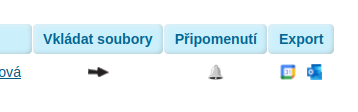
\includegraphics[width=0.33\textwidth]{img/pripomenuti-off.png}
    \caption{Ikona pro připomenutí odevzdáváren v~neaktivním stavu (vlastní zpracování)}
    \label{fig:pripomenuti-off}
\end{figure}

\begin{figure}[H]\centering
    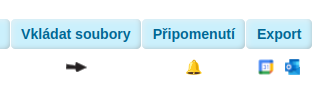
\includegraphics[width=0.33\textwidth]{img/pripomenuti-on.png}
    \caption{Ikona pro připomenutí odevzdáváren v~aktivním stavu (vlastní zpracování)}
    \label{fig:pripomenuti-on}
\end{figure}

Výběr času připomenutí je realizován pomocí dialogového okna, které obsahuje seznam zaregistrovaných časů připomenutí a sadu tlačítek pro registraci dalších časů připomenutí. Uživatelské rozhraní tohoto dialogového okna je možné vidět na obrázku \ref{fig:pripomenuti-modal}, který zobrazuje nastavení pro odevzdávárnu se dvěma již zaregistrovanými časy připomenutí.

\begin{figure}[H]\centering
    
\includegraphics[width=0.66\textwidth]{img/pripomenuti-modal.png}
    \caption{Dialogové okno pro nastavení časů připomenutí (vlastní zpracování)}
    \label{fig:pripomenuti-modal}
\end{figure}

\subsection{Implementace vylepšeného rozvrhu}

Asi nejvíce komplexní částí celého rozšíření je modul pro vylepšený rozvrh, jehož funkce jsou podrobněji popsané v~kapitole \ref{sec:vylepseny-rozvrh}. Tato komplexita vychází především z~množství zpracovávaných informací a z~rozmanitosti uživatelského rozhraní, které se musí flexibilně přizpůsobovat různým situacím. 

Ihned po detekci že se uživatel nachází v~modulu osobní rozvrh dochází k~načtení a zpracování tabulky s~rozvrhem hodin a tabulky s~poznámkami k~hodinám, ze kterých proběhne extrakce informací, podobně jako tomu bylo u~ostatních popisovaných modulů. Jako první proběhne zpracování hodin v~zobrazeném rozvrhu. 

Původní rozvrh poskytovaný informačním systémem InSIS je navržený jako HTML tabulka, která obsahuje sloupce pro každých 5 minut v~časovém okně od 7:30 do 19:30. Každá hodina zanesená v~tomto rozvrhu je reprezentovaná pomocí buňky tabulky, která přesahuje přes počet sloupců odpovídající délce trvání v~minutách děleno pěti. Každá taková buňka je barevně odlišena podle typu rozvrhové akce (zdali se jedná o~přednášku, cvičení nebo blokovou akci). Tato barva je definována pomocí CSS tříd, které jsou aplikovány na buňku a které je možné využít pro extrakci typu každé buňky, respektive každé rozvrhové akce. U~každé z~rozvrhových akcí dochází k~extrakci místnosti, předmětu, vyučujícího, dne v~týdnu, délky trvání, typu rozvrhové akce a času začátku dané akce.

Poté co proběhne zpracování a extrakce informací z~původního rozvrhu dochází k~zpracování poznámek k~rozvrhu, které se nachází ve spodní části obrazovky pod rozvrhem. Klíčovým typem poznámek k~hodinám je definice volných dní, které jsou detekovány pomocí regulárního výrazu. Dalším důležitých typem poznámky jsou datumy konání v~případě, že se jedná o~blokovou akci. Tento typ poznámek se týká především mimosemestrálních kurzů a seminářů, které probíhají pouze v~některých týdnech.

Zpracované informace z~původního rozvrhu a z~poznámek k~rozvrhu jsou následně zkombinovány do pole objektů, obsahující datovou reprezentaci rozvrhových akcí a k~nim přidružené zpracované poznámky. Po spojení dat dochází k~odstranění původního rozvrhu a vytvoření kořenového prvku pro vyrenderování React komponenty s~upraveným rozvrh. Této komponentě jsou jako vstupní parametry předány zkombinovaná data společně s~tokenem pro autentikaci na podpůrném serveru pro načítání uživatelských poznámek v~rozvrhu. Kořenový element obsahuje pouze tuto jedinou komponentu \code{<Timetable/>}, která se následně stará o~celý proces načítání a renderování dat v~rozvrhu.

V~komponentě \code{<Timetable/>} dochází k~načtení poznámek z~podpůrného serveru pomocí technologie AJAX a~vytvoření kontextu pro každý týden výukového období. Tato komponenta je tvořena několika dílčími komponentami. První z~těchto komponent je uživatelské rozhraní pro zobrazení a~přepínání aktuálně zobrazeného týdne. Ve výchozím stavu se zobrazuje aktuální týden, pokud je aktuální den v~týdnu v~rozpětí pondělí - pátek. Pokud je aktuální den sobota nebo neděle, zobrazuje se ve výchozím stavu týden následující po aktuálním týdnu.   

\begin{figure}[H]\centering
    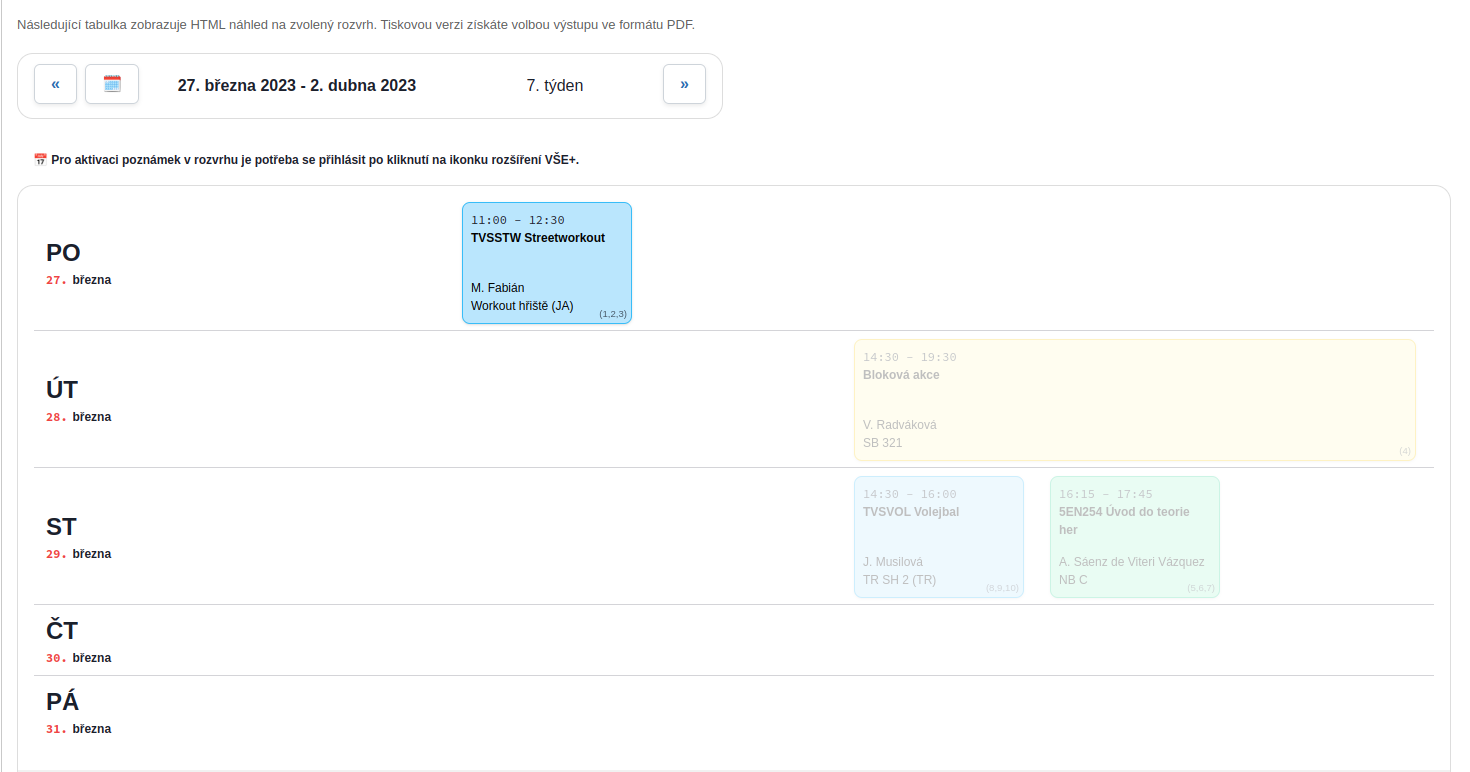
\includegraphics[width=\textwidth]{img/rozvrh-volne-dny.png}
    \caption{Grafické odlišení volných dní v~rozvrhu (vlastní zpracování)}
    \label{fig:rovrh-volne-dny}
\end{figure}

\subsection{Implementace přihlášení do rozšíření}

Přihlášení do webového rozšíření je společně s~nastavením uživatelských preferencí jedinou částí rozšíření, která není implementovaná v~podobě modulu content scriptu. Namísto toho je tato část rozšíření implementovaná jako popup obrazovka, která se zobrazí po kliknutí na ikonu rozšíření jak zobrazují obrázky \ref{fig:prihlaseni-1} a \ref{fig:prihlaseni-2}.

\begin{figure}[H]\centering
    
\includegraphics[width=\textwidth]{img/prihlaseni-vse-plus.png}
    \caption{Popup obrazovka pro zadání emailové adresy (vlastní zpracování)}
    \label{fig:prihlaseni-1}
\end{figure}


\begin{figure}[H]\centering
    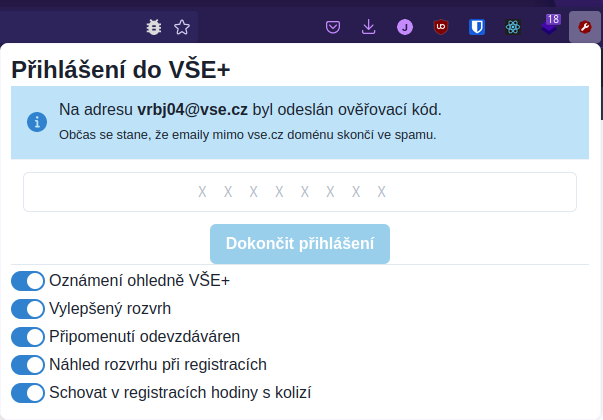
\includegraphics[width=\textwidth]{img/prihlaseni-vse-plus-kod.png}
    \caption{Popup obrazovka pro zadání ověřovacího kódu (vlastní zpracování)}
    \label{fig:prihlaseni-2}
\end{figure}

Tato popup obrazovka je zaregistrovaná v~manifestu rozšíření. Ve verzi 2 manifestu se jedná o~klíč \code{browser\_action}, ve verzi 3 manifestu se jedná o~klíč \code{action}. V~rámci tohoto klíče se definují 2 vlastnosti. První vlastností je \code{default\_popup}, který představuje cestu ke~vstupnímu HTML souboru který se má v~rámci popup obrazovky rozšíření zobrazit. Tato cesta je relativní vůči kořenovému adresáři složky se sestaveným rozšířením a v~případě rozšíření VŠE+ se jedná o~soubor s~názvem \code{popup.html}. Druhou z~vlastností je \code{default\_title}, která představuje nadpis, který se má zobrazit po najetí myší na ikonu rozšíření v~liště prohlížeče.

Soubor \code{popup.html}, na který se v~rámci manifestu odkazuje sekce pro definici popup stránky je velice jednoduchý a~kromě základních definic HTML dokumetu obsahuje pouze 2 důležité části. Jednou částí je definice \code{<div>} elementu, který slouží jako kořenový element pro vložení React aplikace. Další částí jsou importy sestavených JavaScript souborů, které zajistí vykreslení React aplikace v~rámci definovaného kořenového elementu. Prvním importem je soubor \code{js/vendor.js}, který obsahuje kód závislostí a knihoven, zejména kód pro knihovnu React.js a sadu komponent Chakra UI. Druhým souborem je \code{js/popup.js}, který obsahuje zkompilovaný TypeScript kód pro vyrenderování grafického rozhraní pro přihlášení a uživatelské preference společně s~implementací přidružené logiky pro načítání a ukládání uživatelských preferencí, odesílání autentikačních požadavků na podpůrný webový server a ukládání vygenerovaného autentikačního tokenu.

\subsection{Uživatelské preference a aktivace funkcionalit}

Jak je možné vidět na obrázcích \ref{fig:prihlaseni-1} a \ref{fig:prihlaseni-2}, uživatel má možnost si v~rámci popup stránky rozšíření zvolit, které z~přidaných funkcionalit jsou zapnuté a které nikoliv. Tyto preference jsou definované v~rámci React komponenty \url{src/components/Preferences.tsx}, kde jsou součástí objektu s~názvem pro zobrazení pro uživatele.

Celkem je definovaných 5 přepínačů, které je možné vypnout nebo zapnout podle preference uživatele rozšíření. Definice klíčů a přidružených popisů funkcionalit je možné vidět ve výpise \ref{code:preferences-features}

\begin{lstlisting}[
    label={code:preferences-features},
    caption={Definice přepínačů a přidružených popisů funkcionalit (vlastní zpracování)}
]
const names: Record<string, string> = {
    "notifications": "Oznámení ohledně VŠE+",
    "enhanced-timetable": "Vylepšený rozvrh",
    "submission-reminders": "Připomenutí odevzdáváren",
    "timetable-preview": "Náhled rozvrhu při registracích",
    "timetable-preview:hide-collisions":
        "Schovat v~registracích hodiny s~kolizí"
}
\end{lstlisting}

Jak je vidět u~posledního definovaného přepínače, pokud se jedná o~přepínač závislý na jiném přepínači, v~tomto případě konkrétně o~přepínač \url{timetable-preview:hide-collisions}, který je závislý na přepínači \url{timetable-preview}, je klíč přepínače oddělen dvojtečkou, což umožňuje validaci, že funkcionalita, na které je přepínač závislý je zapnutá. V~případě, že daná funkcionalita je uživatelem vypnutá, je zablokována možnost měnit závislé přepínače. Tuto situaci zachycuje obrázek \ref{fig:zavisle-prepinace}, kde je možné vidět zablokování změny přepínače "Schovat v~registracích hodiny s~kolizí", protože přepínač "Náhled rozvrhu při registracích", na kterém je druhý přepínač závislý, se nachází ve vypnutém stavu.

Detekce jestli se jedná o~závislý přepínač a jestli má být zablokována možnost měnit hodnotu se vyhodnocuje pro každý přepínač pomocí kódu ve výpise \ref{code:user-preferences-disabled}.

\begin{figure}[H]\centering
    
\includegraphics[width=0.66\textwidth]{img/zavisle-prepinace.png}
    \caption{Příklad závislého přepínače v~uživatelských preferencích (vlastní zpracování)}
    \label{fig:zavisle-prepinace}
\end{figure}

\begin{lstlisting}[label={code:user-preferences-disabled}, caption={Detekce stavu závislého přepínače (vlastní zpracování)}]
const disabled = feature.includes(":") && !isFeatureEnabled(
    preferences,
    feature.split(":")[0]
)
\end{lstlisting}

Proměnná \code{feature} obsahuje textový řetězec s~klíčem přepínače a proměnná \code{preferences} obsahuje načtené preference uživatele. V~prvním kroce proběhne kontrola, že klíč obsahuje znak dvojtečky a pokud ano, klíč se rozdělí na pole textových řetězců podle dvojtečky. Tedy například u~klíče \code{"timetable-preview:hide-collisions"} by došlo k~rozdělení na pole \code{["timetable-preview", "hide-collisions"]}. Z~tohoto pole se pak vezme první prvek, v~tomto případě \code{"timetable-preview"} a proběhne kontrola, jestli je přepínač s~tímto klíčem přepnutý do vypnutého stavu.


Ukládání a načítání uložených uživatelských preferencí je implementováno prostřednictvím \code{browser.storage}, které bylo zmíněno v~předchozích kapitolách. Při prvním renderu uživatelských preferencí dojde k~načtení uložených hodnot pomocí volání funkce \url{browser.storage.local.get("preferences")}. Pokud nejsou uložené preference nalezeny, je vrácen prázdný objekt, který v~důsledku chování implementace funkce \code{isFeatureEnabled} popsané ve výpise \ref{code:is-feature-enabled} způsobí, že všechny přepínače se nachází v~zapnutém stavu. 

\begin{lstlisting}[label={code:is-feature-enabled}, caption={Definice funkce \code{isFeatureEnabled} (vlastní zpracování).}]
export const isFeatureEnabled = (preferences: Preferences, feature: string): boolean => {
// Fallback to all features enabled by default for discoverability
if (!preferences || !Object.keys(preferences.features).includes(feature)) {
    return true;
}

return preferences.features[feature];
};
\end{lstlisting}

\section{Sestavování a distribuce rozšíření}

Standardním postupem distribuci rozšíření do webových prohlížečů je využití internetových obchodů, které tyto rozšíření nabízí. Tyto obchody jsou většinou spojené přímo s~konkrétním internetovým prohlížečem a jsou provozovány výrobcem internetového prohlížeče. 

Pro distribuci byly zvoleny 2 hlavní internetové obchody s~rozšířeními do webových prohlížečů: Google Web Store a Firefox Addons. Google Web Store je internetový obchod provozovaný společností Google ve kterém jsou k~dispozici rozšíření a témata do webového prohlížeče Google Chrome a ostatních prohlížečů založených na technologii Chromium. 
Výhodou podpory ostatních prohlížečů je, že uživatelé alternativních prohlížečů jako je zejména prohlížeč Opera nebo Microsoft Edge si mohou rozšíření nainstalovat z~obchodu Google Web Store bez nutnosti instalace webového prohlížeče Google Chrome. Druhým zmíněným obchodem, který byl zvolen pro distribuci webového rozšíření VŠE+ je internetový obchod Firefox Addons, který je provozovaný společností Mozilla, která zároveň vyvíjí webový prohlížeč Mozilla Firefox, pro který je tento internetový obchod určen. 

Mezi oběma zmíněnými internetovými obchody existuje celá řada podobností a~rozdílů. Jedním z~prvních rozdílů, se kterými přijde vývojář do styku, je nutnost koupě vývojářské licence pro obchod Google Web Store. Tato licence stojí v~době psaní této práce 5 amerických dolarů a~bez této licence není možné publikovat do obchodu Google Web Store žádný obsah. Naproti tomu publikování webových rozšíření a témat do obchodu Firefox Addons nevyžaduje licenci a~může být realizováno bezplatně.       

Jednou z~výhod využití zmíněných internetových obchodů jsou metriky, které tyto obchody poskutují. Autorům rozšíření dodávají podrobné statistiky o~počtu instalací, demografii uživatelů rozšíření a rozložení nainstalovaných verzí rozšíření. Tyto statistiky je možné vidět v~panelu vývojáře a zmíněné obchody umožňují stažení zdrojových dat v~podobě csv souboru.

\begin{figure}[htbp!]\centering
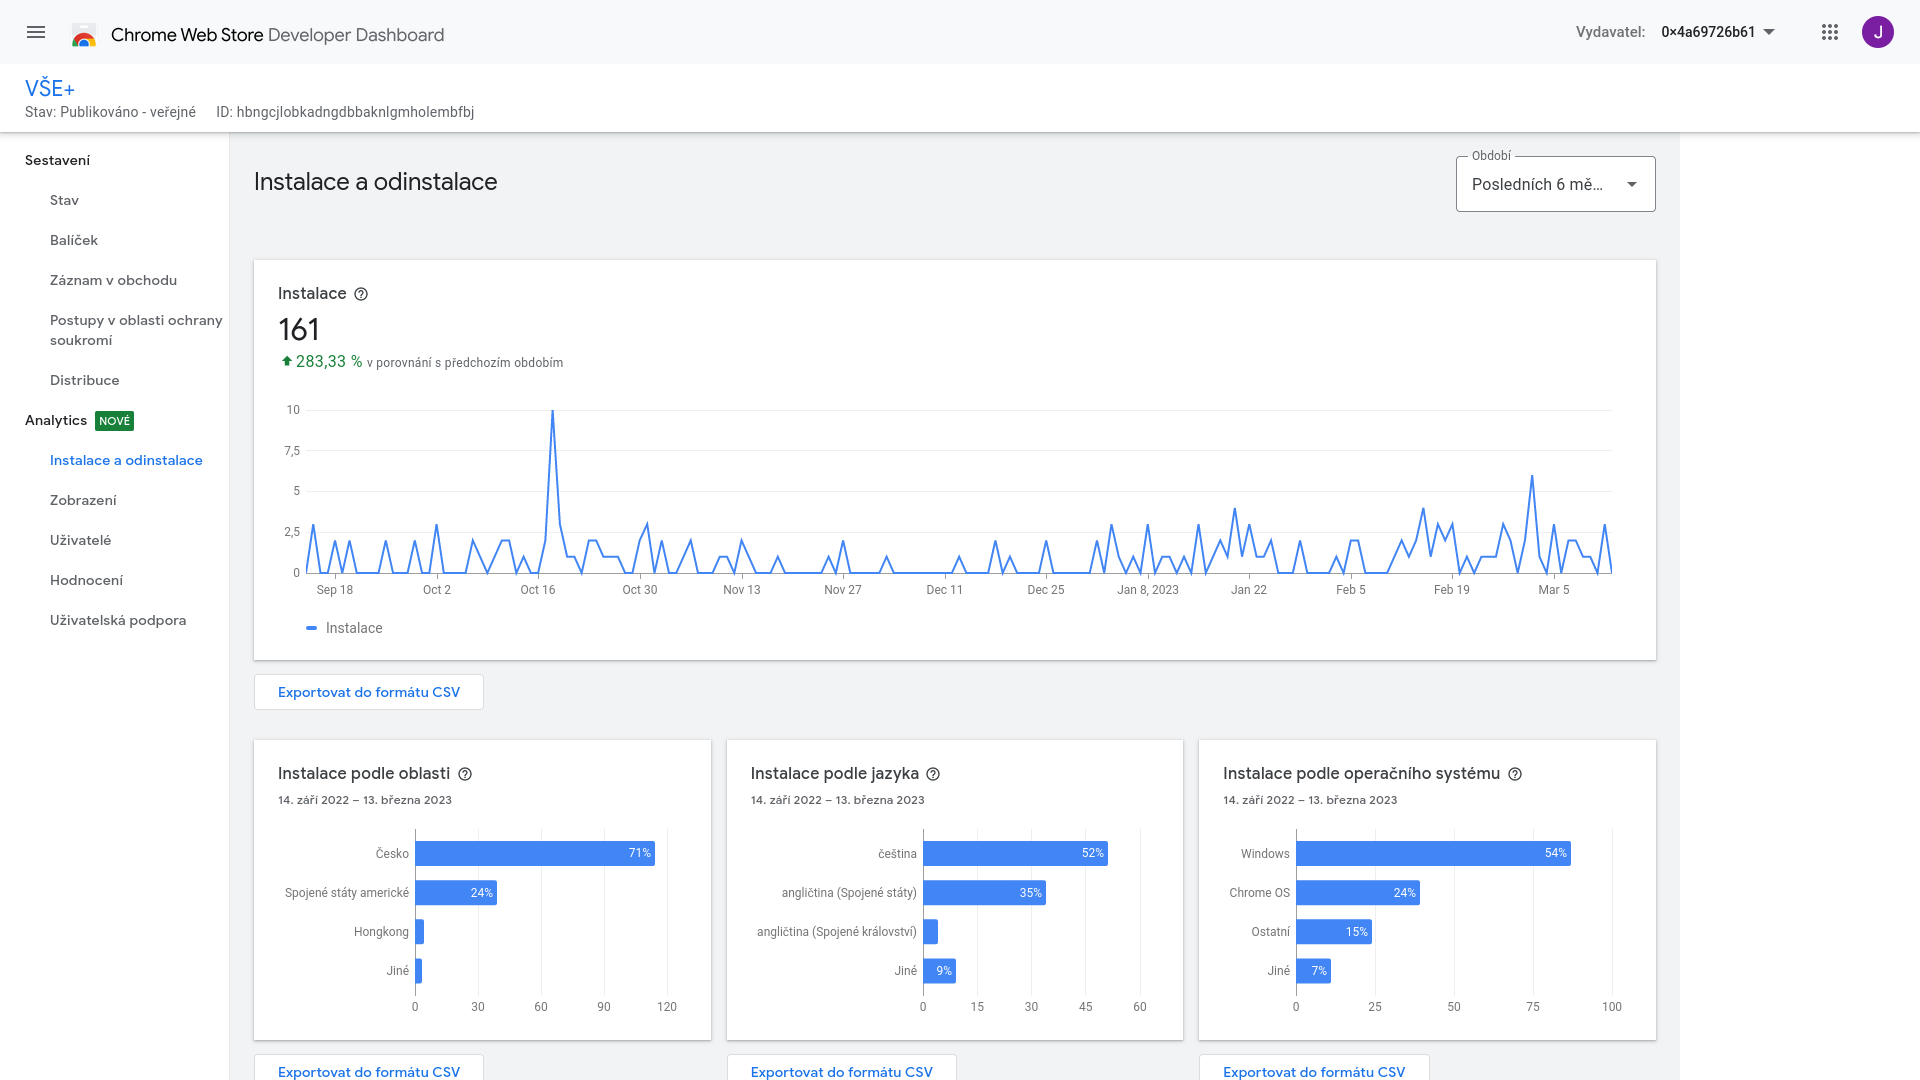
\includegraphics[width=\textwidth]{img/google-webstore-analytics.png}
% Příponu není potřeba explicitně uvádět, pdflatex automaticky hledá pdf.
% Rozměry také není nutné uvádět.
\caption{Statistiky v~panelu vývojáře v~rámci obchodu Google Web Store (vlastní zpracování)}
\label{obr:google-webstore-analytics}
\end{figure}

\subsection{Sestavování balíčků rozšíření}

Před publikací je nutné zkompilovat zdrojový kód společně s~manifestem rozšíření a~ostatními statickými soubory z~adresáře \url{public}. Výstupem sestavení je komprimovaný zip soubor, který v~kořenovém adresáři obsahuje soubor s~manifestem rozšíření a zkompilované zdrojové kódy.

V~rámci sestavování balíčku také dochází k~minimalizaci počtu sestavených souborů. K~tomu slouží takzvané bundlery, které umožňují zkombinovat více souborů do jednoho, který se označuje jako bundle. Dále tyto nástroje umí provést minifikaci výsledného kódu a optimalizaci závislostí. Pro sestavování bundle rozšíření VŠE+ byl zvolen nástroj Webpack, který je v~současnosti jedním z~nejrozšířenějších bundlerů. Jednou z~výhod tohoto bundleru je možnost extenzivní konfigurace pomocí JavaScript kódu, což umožňuje využití konstruktů programovacího jazyka JavaScript jako jsou cykly nebo kopozice funkcí při definici konfiguračních pravidel. Využití těchto syntaktických konstrukcí není monžé u~konfiguračních souborů ve formátech jako je například JSON nebo YAML.

V~rámci projektu jsou definované 2 webpack konfigurace pro sestavování balíčků, jedna pro sestavování během vývoje a jedna pro produkční sestavení. Tyto konfigurace se nachází v~souborech \code{webpack/webpack.dev.js} a \code{webpack/webpack.prod.js}. Dále se ve složce \code{webpack} nachází ještě soubor \code{webpack.common.js}, který obsahuje konfigurační pravidla, která jsou sdílená mezi produkční a vývojářskou verzí konfigurace. Cesta ke zvolenému konfiguračnímu souboru se předává programu \code{webpack} pomocí parametru \code{-{}-config}. Pro snazší práci s~předáváním konfiguračních souborů nástroji webpack byly definovány 2 aliasy v~sekci \code{scripts} souboru \code{package.json}.

\begin{lstlisting}[label={code:package-json-webpack-alias}, caption={Definice aliasů pro práci s~nástrojem webpack (vlastní zpracování)}]
"scripts": {
    "dev": "webpack --config webpack/webpack.dev.js --watch",
    "build": "webpack --config webpack/webpack.prod.js",
}
\end{lstlisting}

Definice aliasů viz výpis \ref{code:package-json-webpack-alias} umožňují sestavení balíčku pomocí nástroje webpack spouštět přes příkazy \code{npm run dev} pro vývojovou konfiguraci, respektive \code{npm run build} pro produkční konfiguraci. Parametr \code{-{}-watch} u~aliasu \code{dev} spustí webpack v~takzvaném watch módu, který spouští kompilaci po změně jakéhokoliv ze souborů, které webpack spravuje. To zásadním způsobem zvyšuje produktivitu při vývoji rozšíření, protože je možné ihned po úpravě zdrojového kódu pozorovat implementované změny bez nutnosti manuálního spouštění kompilace a sestavení balíčku.

Pro zjednodušení a automatizaci sestavování rozšíření do balíčku publikovatelného na zmíněné internetové obchody je využíváno GitLab CI/CD pipeline, která automaticky sestavuje balíčky a vytváří takzvané releases na platformě GitLab, ze kterých je možné tyto sestavené balíčky přímo publikovat na zmíněné internetové obchody s~rozšířeními. 

Zdrojový kód této CI pipeline je možné vidět ve výpise \ref{code:gitlab-ci-pipeline} a snímek obrazovky z~platformy GitLab s~výsledkem běhu je možné vidět na obrázku \ref{fig:extension-gitlab-ci}. 

\begin{figure}[htbp!]\centering
    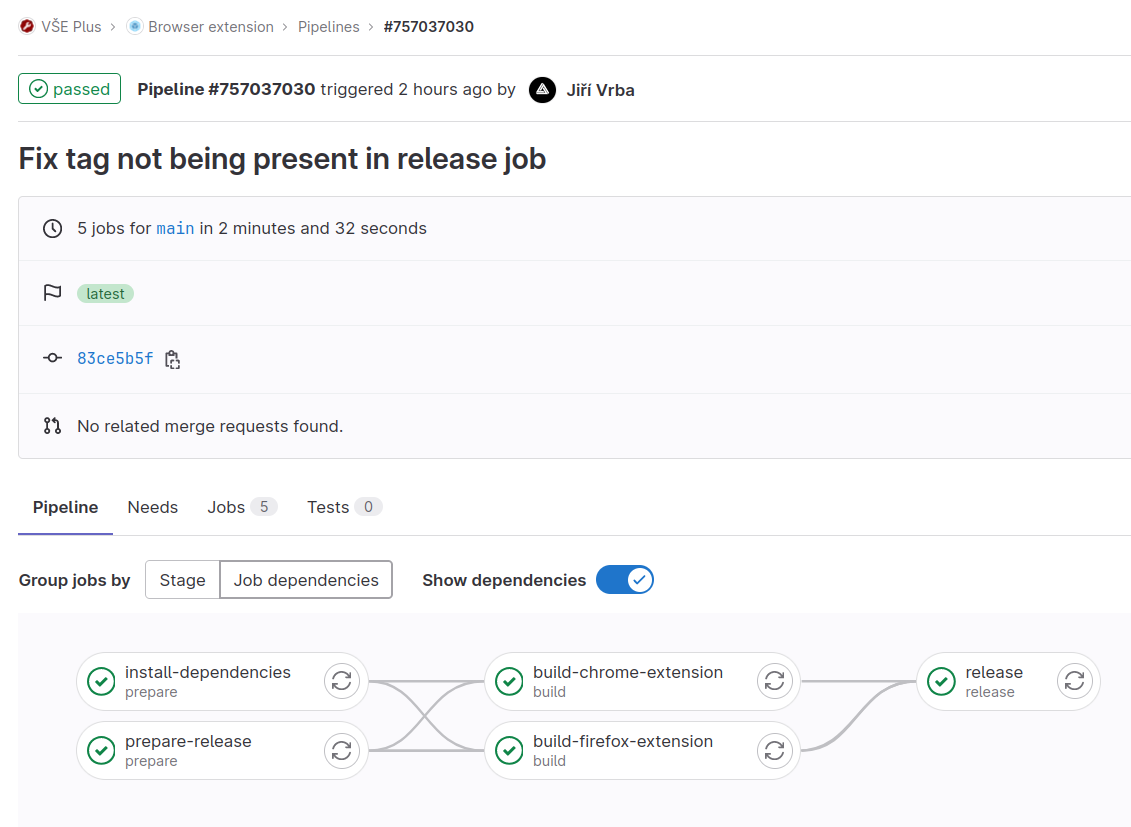
\includegraphics[width=\textwidth]{img/extension-gitlab-ci-pipeline-overview.png}
    \caption{GitLab CI Pipeline (vlastní zpracování)}
    \label{fig:extension-gitlab-ci}
\end{figure}

V~horní části obrázku \ref{fig:extension-gitlab-ci} se nachází informace o~git commitu, pro který se pipeline spouští, a ve spodní části obrázku je vidět graf závislostí jednotlivých úkonů, které se mají v~rámci pipeline spustit.

Aktuální verze kompletního zdrojového kódu včetně historie změn je dostupná v~podobě repozitáře na platformě GitLab na adrese \url{https://gitlab.com/vse-plus/extension}.
